\documentclass[finnish,utf8,nonumbib,palatino,kandi]{gradu2}
\usepackage[utf8]{inputenc}
\usepackage[pdftex]{graphicx}
\usepackage{listings}
\usepackage{color}
\usepackage{qtree}

\makeatletter
\ifgradu@pdf
  \usepackage[pdftex,bookmarksopen,bookmarksnumbered]{hyperref}
%\hypersetup{colorlinks,citecolor=blue}

\else
	\RequirePackage[hypertex]{hyperref}
\fi
\makeatother

\title{MVC-arkkitehtuurin toteutus Pyramid web-sovelluskehyksessä}
\setauthor{Toni Juhani}{Haka-Risku}
\yhteystiedot{tojuhaka@gmail.com}
\translatedtitle{Pyramid-framework and MVC-architecture}
\abstract{This is my english abstract}
\tiivistelma{Toteutuuko MVC-arkkitehtuuri Pyramid-sovelluskehyksessä?}
\keywords{P, NP, complexity theory}
\avainsanat{P, NP, kompleksisuusteoria}

\definecolor{light-gray}{gray}{0.96}

\lstdefinelanguage{Smalltalk}{ 
morekeywords={true,false,self,super,nil}, 
sensitive=true, 
morecomment=[s][\color{blue}]{"}{"}, 
morestring=[d]',
alsoother={_},
style=SmalltalkStyle,
columns=fullflexible,
basicstyle=\ttfamily,
backgroundcolor=\color{light-gray},
xleftmargin=.20in,
showspaces=false,
framexleftmargin=15pt,
tabsize=4
} 
\lstdefinestyle{SmalltalkStyle}{ 
literate={:=}{{$\gets\ $}}2{^}{{$\uparrow$}}1{_}{{$\gets\ $}}2{ä}{{\"a}}2{ö}{{\"o}}2
} 


\begin{document}
\preface

Tutkimuksen aiheen valintaan vaikutti työelämässä saatu
 kokemus web-sovellusten kehittämisestä Python-ohjelmointikielellä. Erityisesti
kokemusta on kertynyt Plone-sisällönhallintajärjestelmästä, josta myös Zope- sekä
Grok-sovelluskehykset ovat tulleet tutuiksi. Kokemuksen kautta on myös herännyt mielenkiinto
muita tarjolla olevia vaihtoehtoja kohtaan, joista tällä hetkellä uusin on Pyramid. Koska suurin osa Python-pohjaisista
web-sovelluskehyksistä käyttää MVC-arkkitehtuuria, on mielenkiinto herännyt myös itse MVC-arkkitehtuuriin. Tästä syystä
tutkimuksessa tarkastellaan MVC-arkkitehtuurin ja Pyramidin suhdetta toisiinsa.

\mainmatter
\section{Sanasto}

\section{Johdanto}
Toteutuuko MVC-arkkitehtuuri Pyramid-sovelluskehyksessä?

\section{Tausta}
Rakentaessamme interaktiivisia sovelluksia, modulaarisilla komponenteilla on paljon etuja. Suunnittelemalla komponentit mahdollisimman erillään toisistaan, helpotetaan
ohjelmistosuunnittelijaa ymmärtämään ohjelmakoodia. Samalla pystytään muuttamaan jotakin tiettyä komponenttia ilman, että tarvitsee tietää paljoakaan muista komponenteista \cite{Krasner:desc}.
MVC-arkkitehtuuri on ohjelmistokehityksessä käytetty rakenne, joka määrää ohjelmakoodin jaottelun kolmeen osaan: Malli(model), Näkymä(view) ja Ohjain(controller). MVC on käytössä monissa sovelluksissa ja erityisesti se on saanut
huomiota web-sovelluskehyksien toteutuksissa. Sovelluskehyksen tehtävänä on tuoda sovelluksen kehitykseen mukaan
taso, joka tarjoaa erilaisia kirjastoja ratkaisemaan yleisimpiä ongelmia. Monet sovelluskehykset kuitenkin esiintyvät "MVC-kehyksinä" TODO: viite, mutta eivät 
todellisuudessa toteuta täysin MVC-arkkitehtuuria sellaisena, kuin se alunperin olisi tarkoitettu. Näistä yleisimpiä sovelluskehyksiä ovat Python-pohjaiset
ja erityisesti ZCA:n (Zope Component Architecture) omaavat kehykset, kuten esimerkiksi Pyramid ja Grok. Syy sille, miksi
kyseiset sovelluskehykset eivät toteuta MVC:tä täysin, on konkreettisen \emph{ohjaimen(controller)} puute. Tällaisten
sovelluskehysten kehittyessä pystytäänkin kyseenalaistamaan koko konkreettisen ohjaimen merkitys MVC-arkkitehtuurissa.
herää kuitenkin kysymys siitä ovatko kyseiset sovelluskehykset MVC-kehyksiä vai eivät? Tämän tutkimuksen tarkoituksena on vastata edellä esitettyyn
kysymykseen Pyramid-sovelluskehyksen näkökulmasta.

\subsection{Aiheen rajaus}
Tutkimuksessa käsiteltävä aihe on rajattu tarkastelemaan Pyramid-sovelluskehystä sekä MVC-arkkitehtuuria. Pyramid-sovelluskehystä
tarkastellaan MVC:n näkökulmasta, joten muihin Pyramidissa käytetyihin tekniikoihin ei oteta kantaa. Pyramidiin on saatavana myös suuret määrät erilaisia lisäosia, joilla saadaan sovelluskehys muokattua tiettyyn tarkoitukseen. Lisäksi lisäosat pystytään toteuttamaan lähes mitä tahansa tekniikkaa käyttäen. Tämän takia on lähes mahdotonta tutkia MVC:n toteutusta kaikkien tekniikoiden näkökulmasta, joten tutkielmassa käsitellään ainoastaan Pyramidin alkuperäistä toteutusta huomioimatta lisäosia.

Tutkimuksessa selvitetään MVC:n sekä web-sovelluskehyksien taustat ennen varsinaista tutkimuskysymyksen käsittelyä. Pääpaino
on kuitenkin MVC:ssä, koska sitä voidaan pohjata hyvin tieteelliseen lähdekirjallisuuteen. Koska tutkimus perustuu
selvittämään korkean tason web-sovelluskehyksen käyttytymistä MVC:n kontekstissa, ei MVC-komponenttejen toteutusta käydä liian teknisesti läpi. Perusajatus kuitenkin komponenttejen suhteista, rakenteesta ja
kommunikaatiosta selvitetään. MVC-arkkitehtuurin toteutukset ohjelmointitasolla sidotaan SmallTalk -ohjelmointikieleen. 
Syy kielen valintaan löytyy MVC-arkkitehtuurin historiasta sekä lähekirjallisuuden tarjoamasta materiaalista. Esitellyt ratkaisut
pätevät kuitenkin mihin tahansa muuhun ohjelmointikieleen, joten kielen valinnalla ei tässä tilanteessa ole merkitystä. \\
Tutkimuksessa käytettyjä termejä ei selitetä erikseen tekstissä, vaan ne löytyvät tutkimuksen sanasto-osiosta.

\section{Kirjallisuuskatsaus}
Kirjallisuuskatsauksessa käydään läpi vaihe vaiheelta, miten lähdemateriaalia kerätään
tutkimusta varten. Lähdemateriaalin haku toteutetaan hakukoneilla, jotka ovat tarkoitettu
erityisesti tieteellisten artikkeleiden etsimiseen. Tässä tutkielmassa käytetyt hakukoneet ovat seuraavat:
IEEE Xplore, ACM Digital Library, Google Scholar jne.(TODO: luettelo käytetyistä hakukoneista) Jokaista tutkimuksessa tutkittavaa
tekniikkaa kohden tehdään erillinen kirjallisuuskatsaus. 

Aluksi muodostetaan kokonaiskuva tuloksista, jolloin silmäillään läpi saatuja artikkeleita. Tässä 
vaiheessa tarkoitus ei ole vielä valita mitään pohjaksi tutkimukselle, vaan kerätä informaatiota
siitä millainen lähdemateriaali on tarjolla kokonaisuudessaan. Saaduista tuloksista poimitaan artikkeleita,
jotka sopivat tutkimuksen aihepiiriin. Seuraavaksi artikkeleista valitaan pohjakirjallisuus tutkimukselle. Tässä vaiheessa artikkelit luetaan huolellisesti
läpi ja varmistutaan siitä, että ne ovat tieteellisesti päteviä tutkimusta varten. Tutkimuksessa esiintyy myös
satunnaisia viittauksia, joita ei ole kirjallisuuskatsauksessa mainittu. Tutkimuksen pääkirjallisuus kuitenkin käydään läpi kirjallisuuskatsauksessa.

Haussa käytetään seuraavia hakutermejä: "MVC" , "MVC Architecture" ja "MVC-Architecture".  Erityisesti
artikkeleita löytyy MVC-arkkitehtuurin soveltamisesta erilaisissa tekniikoissa. Tarkasteltavat artikkelit rajataan kuitenkin niihin, jotka esittelevät suoraan MVC-arkkitehtuuria itseään.  

Google Scholarin puolelta saaduista tuloksista löytyy kaksi artikkelia, jotka sopivat
lähdemateriaaliksi tutkimukseen. Ensimmäinen artikkeleista on John Deaconin kirjoittama artikkeli, joka 
tarkastelee lyhyesti MVC-arkkitehtuuria \cite{Deacon:1995}. Artikkeli on kuitenkin hyvin suppea, mutta
selittää tiivistetysti MVC-arkkitehtuurin idean.  

Toinen artikkeli on Steve Burbeckin kirjoittama, jossa esitellään MVC-arkkitehtuuria sellaisenaan kuin 
sitä käytettiin SmallTalk-80 -rajapinnassa(TODO CHECK) \cite{Burbeck}. Burbeckin artikkeliin viitataan
monissa MVC-arkkitehtuuria käsittelevissä julkaisuissa, joten sen arvo tämän tutkimuksen pohjakirjallisuudessa on vahva. 

Seuraavaksi kartoitetaan pohjakirjallisuutta käyttäen ACM Digital Library sekä IEEE XPlore -hakukoneita. Tuloksista löytyy Glenn E.
Krasnerin kirjoittama julkaisu, missä opetetaan käyttämään MVC-arkkitehtuuria käyttäen Smalltalk-80 kieltä. Julkaisusta löytyi useita versioita, joista tässä tutkielmassa käytetään kumpaakin \cite{Krasner} \cite{Krasner:desc}.  Suurimmaksi osaksi tukeudutaan kuitenkin uudempaan julkaisuun. Tuloksien joukosta
löytyy myös paljon MVC-arkkitehtuuria soveltavia tutkimuksia, jotka eivät suoraan tarkastele MVC-arkkitehtuuria sellaisenaan. Näistä hyvä esimerkki on
Oregonin Yliopistossa kirjoitettu artikkeli kurssista, jossa toteutetaan pienimuotoinen Java-ohjelma käyttäen MVC-Arkkitehtuuria \cite{Morse}. 

Monien MVC-arkkitehtuuria soveltavien artikkeleiden lähdeviitteistä löytyy viittauksia Burbeckin ja Krasnerin artikkeleihin. Tämän perusteella pystytään
toteamaan kyseisten artikkeleiden olevan tieteellisesti päteviä ja tarjoavan kattavan lähdemateriaalin MVC-arkkitehtuurin pohjaksi. 

Lopulta Burbeckin ja Krasnerin kirjoittamien artikkeleiden taustalta löytyy MVC-Paradigman kehittäjä Trygve Reenskaug, jonka omia julkaisuja sekä kotisivujen MVC-osiota
käytetään myös lähteenä tutkimuksessa \cite{Reenskaug}. 

\subsection {Tutkimuksen rakenne}
- Kerrotaan vaihe vaiheelta, miten tutkimuksessa edetään

\section {MVC}
MVC-arkkitehtuurin perusajatus on erottaa käyttöliittymä sovelluslogiikasta ja 
näin tehdä sovelluksesta helposti ylläpidettävä kolmen eri komponentin avulla: 
Malli(Model), Näkymä(View) ja Ohjain(Controller). Jokainen komponentti on 
erikoistunut sovelluksessa johonkin tiettyyn tehtävään. Mallin tehtävänä on 
hallita sovelluksen tilaa ja vastata sen käsittelemästä datasta ohjaimelle ja näkymälle.
Näkymän tehtävänä on taas toteuttaa sovellukselle käyttöliittymä. Ohjaimen tarkoitus on ottaa
vastaan syötteitä käyttäjältä käskien mallia ja näkymää muuttumaan tarvittaessa.  

\begin{figure}[h]
\centering
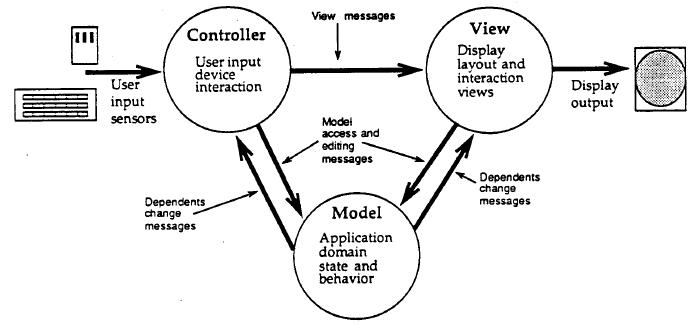
\includegraphics[scale=0.85]{krasner_mvc.jpg}
\caption{Model-View-Controller State and Message Sending \cite{Krasner:desc}}
\end{figure}

Jokaisella komponentilla on oma rajattu tehtävänsä ja ohjelmakoodi tulee jakaa näiden komponenttejen kesken. Jotta MVC-arkkitehtuuria pystytään käyttämään 
tehokkaasti, tulee ymmärtää MVC:n komponenttejen työnjako sekä se kuinka komponentit kommunikoivat keskenään \cite{Burbeck}.  Luodessamme MVC-arkkitehtuurin
toteuttavia komponentteja, tulee ne periä jostakin abstraktista pohjaluokasta(Model, View ja Controller), joka määrittelee kyseisen komponentin käyttäytymisen MVC-arkkitehtuurissa.  Tässä kappaleessa käydään jokainen pohjaluokka erikseen läpi \cite{Krasner:desc}. 

Yleisesti MVC-komponenttejen toimintaa kuvaavassa esimerkissä käyttäjältä tulee jokin syöte, jonka sillä hetkellä aktiivinen ohjain ottaa vastaan ja käskee mallia muuttamaan itseään. Malli puolestaan
tekee sille määrättyjä operaatioita muuttaen tilaansa ja lähettää edelleen viestin muutoksestaan kaikille siihen kiinnitettyille riippuvuuksille (näkymät ja ohjaimet). Näkymät
voivat tämän jälkeen kysyä mallilta sen nykyistä tilaa ja päivittää itsensä, jos siihen on tarvetta. Ohjaimet voivat myös muuttaa tilaansa riippuen mallin tilasta. \cite{Krasner:desc}

\subsection{Historia}

MVC:n esitteli Trygve Reenskaug ollessaan mukana Xerox PARC -tutkimushankkeessa. Ensimmäinen julkaisu MVC:stä
kirjoitettiin vuonna 1978 samassa tutkimuskeskuksessa. Tuolloin julkaisussa esiteltiin kolmen komponentin sijasta neljä
komponenttia: malli(model), näkymä(View), ohjain(Controller) sekä muokkaaja(Editor). Muokkaaja on väliaikainen komponentti, jonka näkymä
luo itsensä ja syötelaitteiden välille. Muokkaaja-komponentista kuitenkin luovuttiin käsitteenä ja se sisällytettiin näkymään ja ohjaimeen. \cite{Reenskaug}.
Alkuperäinen Xerox PARC:n tuottama raportti MVC:stä oli Reenskaugin vuonna 1979 kirjoittama \emph{THING-MODEL-VIEW-EDITOR} \cite{reenskaug:1979}. Raportti 
esitteli MVC-arkkitehtuurin komponentteja käyttäen hyväksi esimerkkejä Kreenskaugin omasta suunnittelutyöstä. Koska MVC:n historia ja suurin osa MVC:n
alkuperäisistä julkaisuista pohjautuvat smalltalk-80 -ohjelmointikieleen, joudutaan väistämättä sitomaan MVC:n tarkastelu smalltalk:iin.  TODO: historia jatkuu 

\subsection{Malli (Class Model)}
Malli pitää yllä sovelluksen tilaa sekä vastaa sovelluksen tallentamasta datasta. Se voi olla esimerkiksi kokonaislukumuuttuja laskuri-sovelluksessa, merkkijono-olio tekstinkäsittelyohjelmassa tai
mikä tahansa monimutkainen olio \cite{Krasner}. Kaikkein yksinkertaisimmassa tapauksessa mallin ei tarvitse kommunikoida ollenkaan ohjaimen ja näkymän kanssa, vaan toimia passiivisena säiliönä datalle. 
Tällaisesta tilanteesta on hyvä esimerkki yksinkertainen tekstieditori, jossa teksti nähdään juuri sellaisena kuin se olisi paperilla. Tässä tapauksessa mallin ei tarvitse ottaa vastuuta
kommunikoinnista näkymälle, koska muutokset tekstiin tapahtuvat käyttäjän pyynnöstä. Tällöin ohjain ottaa vastaan käyttäjän syötteet ja voi esimerkiksi ilmoittaa näkymälle muutoksesta, jolloin näkymä
päivittää mallin. Ohjain voi myös päivittää mallin ja ilmoittaa tästä näkymälle, jolloin näkymä voi pyytää mallin sen hetkistä tilaa. Kummassakaan tapauksesssa mallin ei tarvitse tietää ohjaimen ja näkymän
olemassaolosta \cite{Burbeck}. 

Malli ei kuitenkaan aina voi olla täysin passiivinen. Se voi myös muuttua ilman, että se tarvitsee ohjaimen tai näkymän käskyä. Otetaan esimerkiksi malli, joka muuttaa tilaansa satunnaisin väliajoina. Koska malli muuttaa itse itseään, täytyy sillä olla jokin yhteys näkymään, jotta se voi antaa tiedon muutoksestaan \cite{Burbeck}. Datan kapseloinnin ja ohjelmakoodin uudelleen käytön kannalta ei ole kuitenkaan järkevää, että malli on suoraan yhteydessä näkymään ja ohjaimeen. Ohjaimen ja näkymän tulee siis olla riippuvaisia mallista, mutta ei toisinpäin. Näin mahdollistetaan myös se, että mallilla voi olla useita näkymiä ja ohjaimia \cite{Krasner[s. 27]}.

Yleensä mallin tila muuttuu ohjaimista tulleiden käskyjen kautta. Tämän muutoksen tulisi heijastua kaikkiin näkymiin, jotka ovat sidottuja malliin. Tällaisia tilanteita varten kehitettiin riippuvuudet (\emph{Dependents}).
Riippuvuuksilla tarkoitetaan listaa niistä ohjaimista ja näkymistä, jotka ovat sidottuja malliin. Mallilla tulee siis olla lista riippuvuuksista ohjaimiin ja näkymiin sekä myös kyky lisätä ja poistaa niitä. Malli ei siis tiedä mitään yksittäisistä riippuvuuksista, mutta pystyy kuitenkin lähettämään itsestään muutosviestejä(change messages) listassa oleville ohjaimille ja näkymille. Mallin tuottamat muutosviestit voivat olla minkä tyyppisiä tahansa, joten ohjaimet ja näkymät reagoivat niihin omalla määritellyllä tavallaan  \cite{Krasner[s. 27]}. 

Mallille määritellään pääluokka \emph{Model} ja tälle viitemuuttujan \emph{dependents}, joka viittaa yhteen riippuvaan komponenttiin tai listaan riippuvista komponenteista. Kaikki uudet mallit tulee periä niiden pääluokasta, jotta saavutetaan sama toiminnallisuus kaikkiin mallikomponentteihin. Komponenttejen tieto mallin muutoksista tukeutuu täysin mallin riippuvuusmekanismiin. Kun jokin komponentti luodaan, se rekisteröi itse itsensä malliin riippuvuudeksi ja samalla tavalla se myös poistaa itsensä \cite{Burbeck}.

\subsection{Näkymä (Class View)}
Näkymän tehtävänä on huolehtia graafisesta puolesta MVC-arkkitehtuurista. Näkymä pyytää yleensä mallilta datan ja tämän pohjalta näyttää käyttäjälle käyttöliittymän sovellukseen. Toisinkuin malli, jota pystytään rajoittamattomasti yhdistelemään moniin näkymiin ja ohjaimiin, jokainen näkymä on liitetty yhteen ohjaimeen.  Näkymä siis sisältää viitteen ohjaimeen ja taas ohjain sisältää viitteen näkymään. Kuten ohjain, näkymä on myös rekisteröity mallin riippuvuuksiin. Kummatkin sisältävät siis myös viitteen siihen malliin, johon ne on rekistereröity \cite{Burbeck}. Jokaisella näkymällä on tasan yksi malli ja yksi ohjain \cite{Krasner[s.29]}.  

Näkymä vastaa myös MVC-komponenttejen sisäisestä kommunikaatiosta MVC-kolmikon luontivaiheessa. Näkymä rekisteröi itsensä  riippuvuudeksi malliin, asettaa viitemuuttujansa viittamaan ohjaimeen ja välittää itsestään viestin ohjaimelle. Viestin avulla ohjain rekisteröi näkymän omaan viitemuuttujaansa. Näkymällä on myös vastuu poistaa viitteet sekä rekisteröinnit \cite{Burbeck}. \\
Näkymä ei sisällä ainoastaan komponentteja datan näyttämiseen ruudulla vaan voi sisältää myös useita alanäkymiä(subviews) ja ylänäkymiä(superviews). Tästä muodostuu hierarkia, jossa ylänäkymä hoitaa aina jonkun suuremman kokonaisuuden, kuten esimerkiksi näytön pääikkunan. Alanäkymä taas huolehtii jostain pienemmästä yksityiskohdasta pääikkunassa. Näkymillä on myös viite erilliseen transformaatioluokkaan, joka hoitaa kuvan sovittamisen ja yhdistämisen alanäkymien ja ylänäkymien välillä. Jokaisella näkymällä tulee siis olla protokolla, joka hoittaa alanäkymien poistamisen sekä myös protokolla, jonka avulla näkymän sisäiset transformaatiot tuodaan transformaatioluokalle. Näkymille tarkoitetut viestit kulkevat tämän hierarkian läpi alkaen ylimmästä näkymästä ja päätyen sieltä johonkin alanäkymään, jolle viesti on tarkoitettu. \cite{Krasner:desc} 

\subsection{Ohjain (Class Controller)}
Ohjaimen tehtävänä on ottaa vastaan syötteitä sekä koordinoida malleja ja näkymiä saatujen syötteiden perusteella. Sen tulee myös kommunikoida muiden ohjaimien kanssa. Teknisesti ohjaimessa on kolme viitemuuttujaa: malli, näkymä ja sensori(sensor). Sensorin tehtävänä on toimia rajapintana syötelaitteiden sekä ohjaimen välillä. Sensori mallintaa syötelaitteiden käyttäytymistä ja muuttaa ne ohjaimen ymmärtämään muotoon. 

Ohjaimien tulee käyttytyä siten, että vain yksi ohjain ottaa vastaan syötteitä kerrallaan. Esimerkiksi näkymät pystyvät esittämään informaatiota rinnakkain monen näkymän kautta, mutta käyttäjän toimintoja tulkitsee aina vain yksi ohjain. Ohjain on siis määritelty käyttytymään siten, että se osaa tietyn signaalin perusteella päättää tuleeko sen aktivoida itsensä vai ei. Teknisesti ohjaimen käyttäytymisen määrittelee seuraavat metodit, joiden avulla ohjaimet viestivät \cite{Krasner:desc}. : 
\begin{description}
\item[isControlWanted] \ Tuleeko ohjaimen ottaa hallinta.  
\item[isControlActive] \ Onko ohjain aktiivinen. 
\item[controlToNextLevel] \ Luovutetaan hallinta seuraavalle. 
\item[viewHasCursor] \ Onko ohjaimen näkymässä hiiren kursori. 
\item[controlInitialize] \ Kun ohjain on saanut hallinnan, alustetaan se. 
\item[controlLoop] \ Lähettää \emph{controlActivity} -viesteja niin kauan, kuin ohjaimella on hallinta. 
\item[controlTerminate] \ Lopettaa ohjaimen hallinnan.
\end{description}

Kun ohjain saa hallinnan itselleen, kutsuu se \emph{startUp} -metodia. Metodi kutsuu seuraavia metodeja: \emph{controlInitialize}, \emph{controlLoop} ja \emph{controlTerminate}. Metodit
voidaan ylikirjoittaa, jotta saadaa määriteltyä jokin tietty toiminnallisuus ohjaimelle. Esimerkiksi \emph{controlInitialize} ja \emph{controlTerminate} määräävät mitä tehdään, kun ohjain saa hallinnan tai luovuttaa sen eteenpäin. Ohjaimen hallitessa kutsutaan
\emph{controlLoop} -metodia, joka taas kutsuu \emph{controlActivity} -metodia niin kauan kuin ohjaimella on hallinta.  Metodi \emph{controlActivity} määrää ohjaimen toiminnan hallinnan aikana, joten se ylikirjoitetaan tätä varten. \cite{Krasner:desc}. 


\subsection{Esimerkkiohjelma}
Seuraavaksi esitellään  Dortmundin yliopistossa kirjoitettu yksinkertainen esimerkkiohjelma SmallTalk-80:lla, siitä miten MVC:tä voidaan käyttää
käytännössä. Ohjelmakoodi löytyy myös Krasnerin artikkelista \cite{Krasner:desc}. Ohjelmassa toteutetaan yksinkertainen laskuri-ohjelma, joka käyttää MVC-arkkitehtuuria toteutuksessaan. Ohjelmassa esitellään malli, joka on luokan \emph{Counter} instanssi ja näkymä mikä on luokan \emph{CounterView} instanssi. \emph{Counter} perii mallin ominaisuudet ja 
toimii ohjelmassa yksinkertaisen numero-muuttujan ylläpitäjänä. \emph{CounterView} perii näkymän ominaisuudet ja näyttää mallin (\emph{Counter}) arvon.
Ohjaimena toimiiluokan \emph{CounterController} instanssi, joka perii ohjaimen käyttytymisen. Ohjain tarjoaa sovelluksessa "laatikon", josta voi vähentää
tai lisätä laskurin arvoa. Samanlainen laskuri toteutetaan myös tutkielman Pyramid-osuudessa Pyramidilla, mutta korkeammalla tasolla käyttäen hyväksi
sen tarjoamaa valmista arkkitehtuuria.  \\

Määritellään ensiksi \emph{Counter} -luokka, joka peritään \emph{Model} -luokasta.
\begin{lstlisting}[language=Smalltalk]
Model subclass: #Counter
	instanceVariableNames: 'value'
	classVariableNames: ' '
	poolDictionaries: ' '
  	category: 'Demo-Counter'
\end{lstlisting} 

Seuraavaksi määritellään \emph{Counter} -luokalle metodeita, jotka määrävät
laskuriarvon alustamisen sekä muokkaamisen. Näin kaikki \emph{Counter}-instanssit
lähettävät ja vastaanottavat viestejä samalla tavalla.

\begin{lstlisting}[language=Smalltalk]
Counter methods For: 'Initialize-release' 
Initialize
	"Aseta alkuarvoksi 0"
	self value: 0
Counter methodsFor: 'accessing' 
value
	"Palauta mallin arvo" 
   	^value
value: aNumber
	"Aseta mallin arvo"
	value <- aNumber.
	self changed "to update displayed value"
Counter methodsFor: 'operations' 
decrement
	"Vähennä mallin arvoa yhdellä." 
	self value: value -1
Increment
	"Lisää mallin arvoa yhdellä." 
	self value: value + 1
\end{lstlisting} 

Lisätään luokkaan metodi, jolla itse luokasta saadaan muodostettua instanssi.

\begin{lstlisting}[language=Smalltalk]
Counter class methodsFor: 'instance creation'
new
	"Palauta uusi instanssi luokasta"
	^super new initialize 
\end{lstlisting} 

Seuraavaksi määritellään ohjain (\emph{CounterController}), joka peritään
\emph{Controller} luokasta. Luodaan myös ohjaimelle metodit, joiden avulla
ohjataan mallia sekä näkymää. Metodeissa toteutetaan valikko, joka tarjoaa
mahdollisuuden joko vähentää tai lisätä laskurin arvoa. Kaikki \emph{CounterController} -luokassa käytetyt 
määrittelemättömät muuttujat peritään yliluokasta.

\begin{lstlisting}[language=Smalltalk]
Mouse MenuController subclass: #CounterControIler
	instanceVariableNames: ' '
  	classVariableNames: ' '
  	poolDictionaries: ' '
  	category: 'Demo-Counter'
CounterController methodsFor: 'initialize-release'
initialize
	"Alusta valikko, jossa on mahdollisuus vähentää tai lisätä"
	"mallin arvoa"
  	super initialize.
  	Self yellowButtonMenu: (PopUpMenu labels: 'Increment\Decrement' withCRs)
  	yellowButtonMessages: #(increment decrement)
CounterController methodsFor: 'menu messages'
decrement
	"Vähennä mallin arvoa yhdellä."
 	self model decrement
increment
	"Lisää mallin arvoa yhdellä"
	self model increment
CounterController methodsFor: 'control defaults'
isControlActlve
	"Ota hallinta kun sinistä nappia ei paineta"
	^super isControlActive & sensor blueButtonPressed not
\end{lstlisting} 

Määrätään näkymä (\emph{CounterView}), joka peritään \emph{View} -yliluokasta. Määrätään
myös näkymälle metodit, joiden avulla näytetään mallin tila ruudulla.

\begin{lstlisting}[language=Smalltalk]
View subclass: #Counterview
	instanceVariableNames: ''
	classVariableNames: ''
	poolDictionaries: ''
	category: 'Demo-Counter'

CounterView methodsFor: 'displaying'
displayView
	"Näytä mallin arvo näkymässä"
	| box pos displayText |
	box := self insetDisplayBox.
	"Asettele teksti näkymään. Asettelu ei
	 ole tutkielman kannalta oleellista."
	pos := box origin + (4 @ (box extent y / 3)).
	displayText := ('value:', self model value printString) 
					asDisplayText.
	displayText displayAt: pos
\end{lstlisting} 

Määritellään \emph{update} -metodi, jotta näkymä pystyy päivittämään itsensä. Metodia kutsutaan
yleensä mallin tilan muuttuessa.
\begin{lstlisting}[language=Smalltalk]
CounterView methodsFor: 'updating' 
update: aParameter
  "Yksinkertaisesti päivitä näyttö uudestaan" 
  self display
\end{lstlisting} 
Luodaan myös metodi, joka palauttaa näkymään liitetyn ohjaimen.
\begin{lstlisting}[language=Smalltalk]
CounterView methodsFor: 'controller access'
defaultControllerClass
	"Palauta näkymään rekisteröity ohjain"
	^CounterController
\end{lstlisting} 

Lopuksi tarvitaan metodi, joka luo uuden näkymän sekä rekisteröi mallin ja ohjaimen itseensä. Näkymä näyttää ruudulta 
samalta kuin kuvassa 2.
\begin{lstlisting}[language=Smalltalk]
CounterView class methodsFor: 'instance creation'
open
	"Avaa näkymän uudelle laskurillesovellukselle. Tässä metodissa nähdään
	 kuinka näkymä huolehtii mallin rekisteröinnistä sekä nähdään
	 kuinka näkymiä voi olla useita sisäkkäin."
	| aCounterView topView |
	"Luo laskurinäkymälle uusi näkymä, joka näyttää laskurin arvon"
	aCounterView := CounterView new 
	"Asetetaan malliksi Counter -luokan instanssi"
	model: Counter new.
	aCounterView borderWidth: 2.
	aCounterView insideColor: Form white.
	"Asetetaan ylimmäksi näkymäksi StandardSystemView -luokan
	 instanssi, joka vastaa perinteistä ikkunointimallia"
	topView := StandardSystemView new 
		label: 'Counter'. 
	topView minimumSize: 80@40. 
	"Lisätään edellä luotu laskurinäkymä ylinäkymän alanäkymäksi"
	topView addSubView: aCounterView.
	"Käynnistetään ohjain"
	topView controller open
\end{lstlisting} 

\begin{figure}[h]
\centering
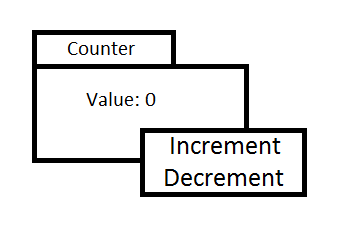
\includegraphics[scale=0.85]{counter.png}
\caption{Kuva CounterView -näkymästä \cite{Krasner:desc}}
\end{figure}

\section{Pyramid}
Pyramid on Python-pohjainen web-sovelluskehys, jonka tehtävänä on helpottaa web-kehitystä tarjoamalla
kehittäjälle valmiita työkaluja avuksi kehitykseen. 

\subsection{Tausta}
Sovelluskehyksen tehtävänä on tuoda sovelluksen kehitykseen mukaan
taso, joka tarjoaa erilaisia kirjastoja ratkaisemaan yleisimpiä ongelmia, joita tulee vastaan sovelluksen kehityksen aikana. Näin vältetään
jo ratkaistujen perusoperaatioiden toistoa ja pystytään keskittymään suoraan sovelluksen toteuttamiseen. Web-sovelluskehykset ovat erityisesti suunnattuja
web-sovellusten ja -palvelujen toteuttamiseen\cite{Frameworks}.  Tärkein ero sovelluskehyksen ja kirjaston välillä on se, että kirjaston ohjelmakoodi kutsustaan aina
kehittäjän toimestaa. Sovelluskehyksessä taas kehittäjän ohjelmakoodia kutsutaan aina sovelluskehyksen toimesta \cite{Pyramid:intr}.

\subsection{Sisältö}
Pyramid on suunniteltu siten, että kehittäjän ei tarvitse tietää suuria määriä erilaisia malleja ja tekniikoita pystyäkseen tuottamaan web-sovelluksia. Se ei myöskään pakota käyttämään kehityksessä
mitään erityisiä tekniikoita, vaan pyrkii olemaan mahdollisimman yksinkertainen ja helposti laajennettavissa erilaisiin käyttötarkoituksiin. Laajentamisella tarkoitetaan erilaisten lisäosien
liittämistä Pyramidiin. Yksinkertaisuuden ja mimimaalisuuden ansiosta se on myös nopeampi kuin monet muut Python-pohjaiset web-sovelluskehykset. Tämä johtuu Pyramidin poikkeuksellisen
pienestä kutsupinosta (\cite{Stack Trace} ajamisen aikana \cite{Pyramid:intr}. TODO: stack trace viite

Koska Pyramid tarjoamaan ainoastaan  välttämättömimmät työkalut web-kehitykseen, Pyramidin kehittäjät
ovat päätyneet web-kehityksessä neljään yleisimpään ongelmaan ja tarjoavat niihin ratkaisun Pyramidissa: 

\begin{description}
\item [URL Mapping] \ URL:ien liittäminen ohjelmakoodiin. 
\item[Template] \ Tuodaan sovelluksen näkymä selaimelle käyttäen HTML-kuvauskieltä (TODO: sanastoon), jolla määrätään näkymän rakenne. Tämän avulla pystytään erottamaan käyttöliittymä sovelluslogiikasta tehokkaasti.
\item[Security] \ Perinteiset tietoturvaongelmat tulee olla ratkaistuna valmiiksi jo sovelluskehyksessä. Tämä ei kuitenkaan tarkoita sitä, että kehittäjä voisi täysin unohtaa tietoturvan merkityksen.
\item[Static Assets] \ Staattisien resurssejen jakaminen niille tarkoitettuihin paikkoihin tiedostorakenteessa.
\end{description}

Yllä määritellyjen neljän pääongelman lisäksi Pyramid tarjoaa lisäosien kautta monia erilaisia työkaluja, joiden avulla pystytään laajentamaan sen ominaisuuksia \cite{Pyramid:intr}. Tutkielman aiheen rajauksen vuoksi ei kuitenkaan
käydä läpi yksityiskohtaisemmin Pyramidin toteutusta ja siihen liitettävissä olevia lisäosia, vaan keskitytään tarkastelemaan MVC:n toteutusta Pyramidissa. 

\subsection{Tiedostorakenne}
Kuten monissa web-sovelluskehyksissä, jaetaan sovelluslogiikka erillisiin tiedostoihin. Näin jokaisella ohjelmakoodilla on oma paikkansa ja sovelluksen hallinta kehityksen aikana helpottuu. Samalla
sovelluskehys löytää tarvittavat asiat oikeista paikoista. Seuraavassa kuvassa esitellään yksinkertaisen web-sovelluksen rakenne Pyramidissa:

\Tree  [.Sovellus !\qsetw{0.6pt} [ kuva.png tyyli.css ].static  [ template.pt ].templates \_\_init\_\_.py views.py models.py ]

Ilman tiedostopäätettä olevat lehdet ovat kansioita, jotka sisältävät muita tiedostoja. Tiedostot \emph{models.py}, \emph{views.py} ja \emph{\_\_init\_\_.py} ovat Python-moduuleita, jotka sisältävät
sovelluksen ohjelmakoodin. Yksinkertaistettuna \emph{\_\_init\_\_ .py}:ssä yhdistetään URL:t ohjelmakoodin sekä sidotaan \emph{template} -tiedostot näkymiin. Pyramidissa näkymien ohjelmakoodi on määritelty views.py -tiedostossa ja 
mallit luodaan \emph{models.py} -tiedostossa.  Kansion \emph{static} sisällä ovat kaikki staattiset resurssit, joita käytetään sovelluksessa. Staattisia resursseja voivat olla esimerkiksi kuva-, ääni- tai tyylitiedostot.
Kansion \emph{templates} alta löytyvät kaikki \emph{template}-tiedostot, jotka määräävät sovelluksen näkymän selaimessa. Tässä tutkielmassa mielenkiinto on kuitenkin kohdistettu \emph{views.py}, \emph{models.py} ja \emph{template.pt}
-tiedostoihin, koska ne sisältävät tarvittavat toteutukset MVC:n tarkasteluun.

\begin{description}
\item [views.py] \ URL:ien liittäminen ohjelmakoodiin. 
\item[Template] \ Tuodaan sovelluksen näkymä selaimelle käyttäen HTML-kuvauskieltä (TODO: sanastoon), jolla määrätään näkymän rakenne. Tämän avulla pystytään erottamaan käyttöliittymä sovelluslogiikasta tehokkaasti.
\item[Security] \ Perinteiset tietoturvaongelmat tulee olla ratkaistuna valmiiksi jo sovelluskehyksessä. Tämä ei kuitenkaan tarkoita sitä, että kehittäjä voisi täysin unohtaa tietoturvan merkityksen.
\item[Static Assets] \ Staattisien resurssejen jakaminen niille tarkoitettuihin paikkoihin tiedostorakenteessa.
\end{description}


\section{MVC \& Pyramid}
Pyramidin kehittäjien dokumenteissa esitellään Pyramid MVC-kehyksenä, mutta samalla myös kyseenalaistetaan tämä väite \cite{Pyramid:intr}. Erityisesti ongelman tuo konkreettisen ohjaimen puute.

\subsection{Näkökulman rajaaminen}
Tässä tutkielmassa keskitytään Pyramidin alkuperäiseen toteutukseen eikä lisäosien tarjoamiin erilaisiin tekniikoihin ja toteutuksiin oteta kantaa. Tämä on tutkielman kannalta tärkeää, koska kaikkien
mahdollisten lisäosien tuomien tekniikoiden tukiminen olisi lähes mahdotonta. Näin tutkielma pysyy myös kandidaatin tutkielman rajoissa.

Pyramidin sovellusarkkitehtuuri on toteutettu käyttäen pohjana MVC-arkkitehtuurin ideaa. Tämä ei kuitenkaan tarkoita sitä, että Pyramid toteuttaisi MVC:n teknisesti sellaisena kuin esimerkiksi Krasner määrittelee \cite{Krasner:desc}. Teknisyydellä
tarkoitetaan tässä kontekstissa tarkkoja MVC-komponenttejen kommunikointisääntöjä sekä ohjelmointiteknisiä ratkaisuja, kuten esimerkiksi abstraktejen yliluokkien toteutuksia. Web-ohjelmointi tuo itsessään jo rajoituksia MVC-komponenttejen kommunikaatiolle
Pyramidissa. Esimerkiksi pyyntö(request) tulee suorittaa aina, jos palvelimelta halutaan tuoda dataa selaimelle \cite{Web}. Tämän perusteella malli ei voi viestittää muutoksestaan näkymälle ja ohjaimelle ilman niiden kautta tulevaa pyyntöä. Tämä rajoittaa mallin viestimistä ohjaimelle ja näkymälle. Tästä syystä Pyramidin MVC-toteutusta ei tarkastella liian teknisestä näkökulmasta, vaan keskitytään korkeamman tason toteutukseen. 
Tutkielman keskittyy tarkastelemaan erityisesti ohjaimen toteutusta Pyramidissa. Koska ohjainta ei ole konkreettisesti määritelty, selvitetään millä tavalla se toteutuu Pyramidissa. Samalla tutkitaan voidaanko Pyramid luokitella MVC-arkkitehtuuriksi tämän perusteella. 

\subsection{Päätelmät (TODO: Nimeä paremmin}


Tässä osiossa tarkastellaan MVC:n kannalta kolmea oleellisinta tiedostoa Pyramidissa: \emph{views.py}, \emph{models.py} ja \emph{template.pt}. Tutkimuksen helpottamiseksi toteutetaan samanlainen laskurisovellus kuin tutkimuksen MVC-osiossa käyttäen
hyvä  




tutkielmassa ei tarkastella MVC:tä liian tarkasti teknisen toteutuksen näkökulmasta, vaan keskitytään korkeamman tason toteutukseen. 

malli ei voi kertoa muutoksestaan näkymälle, vaan näkymä pyytä aina mallilta datan. Tämä tapahtuu


 Web-ohjelmointitekniikat tuovat jo itsessään rajoitteita 
sovelluskehyksessä toteutettujen MVC-komponenttejen kommunikoinnille. 
 

Näin tarkkoihin yksityiskohtiin ei kuitenkaan 

 Web-ohjelmointitekniikat tuovat jo itsessään rajoitteita 


 Krasnerin toteuttama malli MVC:n käytöstä on sidottu yksittäiseen kieleen, joten ohjelmistoteknisiin yksityiskohtiin ei ole tutkielman kannalta järkevää kiinnittää liikaa huomiota.
Tukielma keskittyykin
 Kun tarkastelemme MVC:n toteutusta Pyramidissa, tulee tarkastelu

 Ohjelmistoarkkitehtuurin tarkastelu jossain tietyssä kontekstissa tuo paljon ongelmia. Erityisesti kokoajan muuttuvien ohjelmistotyökalujen myötä yksityiskohtainen
tekninen tarkastelu on hyvin hankalaa. 

 Pintapuolisesti tarkasteltuna Pyramidissa toteutuu MVC hyvin pelkistetyllä tasolla. 
 Malli toteutetaan riippumattomana muista komponenteista ja samalla näkymä

Tämä ei kuitenkaan tarkoita sitä, että Pyramid toteuttaisi MVC:tä juuri sellaisena kuin se Smalltalkissa on alunperin määritelty. Myös
Pyramidin dokumentaatiossa kyseenalaistetaan 




 Web-kehitys
itsessään tuo jo rajoitteita alkuperäisen MVC:n toteutukselle. Erityisesti 

- Näkymä ei voi käskeä mallia muuttumaan, jos views.py määritellään ohjaimeksi. Taas jos ei määritellä nii sittten onnistuu, mutta taas silloin ei ole ohjainta
- näkymä ei voi käskeä mallia, vaan joutuu tekemään sen aina "näkymä-metodin" kautta. Onko näkymä-metodi siis ohjaimen roolissa vai ei?
- Näkymä/Controller joutuu aina kysymään mallilta datan
- Asiakas-palvelin mallin takia ei onnistu
- http protokollan lyhyt selvitys
- web pohjaisen kehityksen luonne
- MVC:n näkökulmasta mielenkiintoisin rakenne löytyy models.py ja views.py tiedostoista sekä template
- Pyramid käyttää yhtä MVC-arkkitehtuurikomponenttia hoitamaan webbisovellusta
- esimerkissä käytetään sqlalchemyn pohjalle tehtyä mallia
- url dispatch
- koska pyramid ei sido mihinkään erityiseen tekniikkaan, käytetään esimerkkinä sqlalchemy ja url dispatch
- Esimerkki voitaisiin toteuttaa "hienommin" esimerkiksi ajaxilla, mutta tämä ei ole tukielman kannalta tärkeää. Vaikka
asynkroninen toteutustapa on nätinpi, ei se silti mene sen lähemmäksi MVC:n alkuperäistä toteutusta. Tämä siksi,
koska näkymä joutuu kuitenkin "pommittamaan" mallia. Mallin tulisi kertoa itsestään mutta se ei toimi.
- MVC-arkkitehtuuria tarkastellaan suoraan pyramidin pohjalta, ei siis oteta kantaa esim javascriptin tuomiin 
toteutuksiin.
- Tutkitaan views.py:tä koska se on kaikkein mielenkiintoisin. Malli on hyvin selkeä, joten siihen ei tarvitse puuttuareq	u

- TODETAAN ETTÄ EMME VOI TUTKIA YKSITYISKOHTAISIEN TEKNISTEN TOTEUTUKSIEN POHJALTA, KOSKA WEB-KEHitYS ON NIIN ERILAISTA. TARKASTELLAAN
SIIS YLEISEMMÄLLÄ TASOLLA PYRAMIDIN MVC-TOTEUTUSTA. ELI SE KONTROLLERI PUUTTUU

- keskitytään vain pyramidin coreen, joten jätetään kaikki ylimääräiset tekniikat pois


 jota pystytään laajentamaan juuri sellaiseksi
kuin kehittäjä itse haluaa. 



\section{Tulokset}
- Lyhyesti tutkimuksen tulokset eri ominaisuuksien pohjalta


---------------------------------------------------------------------------------
Seuraavaksi tutkielmassa esitellään saadut tutkimustulokset, lyhyesti
ja ytimekkäästi (mutta selkeästi).

\section{Tarkastelu}
\subsection{MVC ja Pyramid}
- Onko minkään ominaisuuden kannalta parempi? \\
- Tuovatko ominaisuudet Pyramidiin jotain ainutlaatuista?

\section{Johtopäätökset}
- Mitä voidaan päätellä tuloksista?
------------------------------------------------------------------------------
Lopuksi lyhyessä johtopäätösosassa kerrotaan tutkimuksen pihvi.


\bibliographystyle{finplain} % tai joku muu, sovi ohjaajasi kanssa
\bibliography{esim}

\appendix
\section{Ensimmäinen liite}
\section{Toinen liite}


\section{Lähteet}

\begin{thebibliography}{9} % alle 10 lähdeteosta
\bibitem{Deacon:1995}
    John Deacon Computer Systems Development, Consulting \& Training
    \emph{Model-View-Controller (MVC) Architecture},
    August 1995, revised August 2000, April 2005 and May 2009
\bibitem{Burbeck}
   Burbeck, S.
  \emph{“How to use Model-View-Controller (MVC)”,}
  http://st-www.cs.illinois.edu/users/smarch/st-docs/mvc.html
 
 \bibitem{Krasner}
   Glenn E. Krasner \& Stephen T. Pope
  \emph{“A Cookbook for Using the Model-View-Controller User Interface Paradigm in Smalltalk-80”,}
http://www.ics.uci.edu/~redmiles/ics227-SQ04/papers/KrasnerPope88.pdf

 \bibitem{Krasner:desc}
   Glenn E. Krasner \& Stephen T. Pope
  \emph{A Description of the Model-View-Controller User Interface Paradigm in the Smalltalk-80 System}
   http://www.create.ucsb.edu/~stp/PostScript/mvc.pdf

 \bibitem{Reenskaug}
  XEROX PARC 1978-79
  \emph{MVC XEROX PARC 1978-79}
http://heim.ifi.uio.no/~trygver/themes/mvc/mvc-index.html

 \bibitem{Reenskaug:1979}
  XEROX PARC 1979
  \emph{THING-MODEL-VIEW-EDITOR}
   http://heim.ifi.uio.no/~trygver/1979/mvc-1/1979-05-MVC.pdf

 \bibitem{Reenskaug:2007}
  XEROX PARC 1979
  \emph{The Original MVC reports}
 http://heim.ifi.uio.no/~trygver/2007/MVC\_Originals.pdf

 \bibitem{Frameworks}
Irena Petrijevcanin Vuksanovic, Bojan Sudarevic
  \emph{Use of Web Application Frameworks in the Development of Small Applications}


 \bibitem{Pyramid:intr}
  \emph{Pyramid Introduction}
   http://www.kemeneur.com/clients/pylons/docs/pyramid/narr/introduction.html

\bibitem{Web}
\emph{Research on Web Instant Messaging Using REST Web Service}
http://ieeexplore.ieee.org/stamp/stamp.jsp?arnumber=05607397


\end{thebibliography}

\end{document}
